\documentclass[twoside]{book}

% Packages required by doxygen
\usepackage{fixltx2e}
\usepackage{calc}
\usepackage{doxygen}
\usepackage[export]{adjustbox} % also loads graphicx
\usepackage{graphicx}
\usepackage[utf8]{inputenc}
\usepackage{makeidx}
\usepackage{multicol}
\usepackage{multirow}
\PassOptionsToPackage{warn}{textcomp}
\usepackage{textcomp}
\usepackage[nointegrals]{wasysym}
\usepackage[table]{xcolor}

% Font selection
\usepackage[T1]{fontenc}
\usepackage[scaled=.90]{helvet}
\usepackage{courier}
\usepackage{amssymb}
\usepackage{sectsty}
\renewcommand{\familydefault}{\sfdefault}
\allsectionsfont{%
  \fontseries{bc}\selectfont%
  \color{darkgray}%
}
\renewcommand{\DoxyLabelFont}{%
  \fontseries{bc}\selectfont%
  \color{darkgray}%
}
\newcommand{\+}{\discretionary{\mbox{\scriptsize$\hookleftarrow$}}{}{}}

% Page & text layout
\usepackage{geometry}
\geometry{%
  a4paper,%
  top=2.5cm,%
  bottom=2.5cm,%
  left=2.5cm,%
  right=2.5cm%
}
\tolerance=750
\hfuzz=15pt
\hbadness=750
\setlength{\emergencystretch}{15pt}
\setlength{\parindent}{0cm}
\setlength{\parskip}{3ex plus 2ex minus 2ex}
\makeatletter
\renewcommand{\paragraph}{%
  \@startsection{paragraph}{4}{0ex}{-1.0ex}{1.0ex}{%
    \normalfont\normalsize\bfseries\SS@parafont%
  }%
}
\renewcommand{\subparagraph}{%
  \@startsection{subparagraph}{5}{0ex}{-1.0ex}{1.0ex}{%
    \normalfont\normalsize\bfseries\SS@subparafont%
  }%
}
\makeatother

% Headers & footers
\usepackage{fancyhdr}
\pagestyle{fancyplain}
\fancyhead[LE]{\fancyplain{}{\bfseries\thepage}}
\fancyhead[CE]{\fancyplain{}{}}
\fancyhead[RE]{\fancyplain{}{\bfseries\leftmark}}
\fancyhead[LO]{\fancyplain{}{\bfseries\rightmark}}
\fancyhead[CO]{\fancyplain{}{}}
\fancyhead[RO]{\fancyplain{}{\bfseries\thepage}}
\fancyfoot[LE]{\fancyplain{}{}}
\fancyfoot[CE]{\fancyplain{}{}}
\fancyfoot[RE]{\fancyplain{}{\bfseries\scriptsize Generated by Doxygen }}
\fancyfoot[LO]{\fancyplain{}{\bfseries\scriptsize Generated by Doxygen }}
\fancyfoot[CO]{\fancyplain{}{}}
\fancyfoot[RO]{\fancyplain{}{}}
\renewcommand{\footrulewidth}{0.4pt}
\renewcommand{\chaptermark}[1]{%
  \markboth{#1}{}%
}
\renewcommand{\sectionmark}[1]{%
  \markright{\thesection\ #1}%
}

% Indices & bibliography
\usepackage{natbib}
\usepackage[titles]{tocloft}
\setcounter{tocdepth}{3}
\setcounter{secnumdepth}{5}
\makeindex

% Hyperlinks (required, but should be loaded last)
\usepackage{ifpdf}
\ifpdf
  \usepackage[pdftex,pagebackref=true]{hyperref}
\else
  \usepackage[ps2pdf,pagebackref=true]{hyperref}
\fi
\hypersetup{%
  colorlinks=true,%
  linkcolor=blue,%
  citecolor=blue,%
  unicode%
}

% Custom commands
\newcommand{\clearemptydoublepage}{%
  \newpage{\pagestyle{empty}\cleardoublepage}%
}

\usepackage{caption}
\captionsetup{labelsep=space,justification=centering,font={bf},singlelinecheck=off,skip=4pt,position=top}

%===== C O N T E N T S =====

\begin{document}

% Titlepage & ToC
\hypersetup{pageanchor=false,
             bookmarksnumbered=true,
             pdfencoding=unicode
            }
\pagenumbering{alph}
\begin{titlepage}
\vspace*{7cm}
\begin{center}%
{\Large Parker D\+A\+GD 340 \\[1ex]\large 0.\+1 }\\
\vspace*{1cm}
{\large Generated by Doxygen 1.8.13}\\
\end{center}
\end{titlepage}
\clearemptydoublepage
\pagenumbering{roman}
\tableofcontents
\clearemptydoublepage
\pagenumbering{arabic}
\hypersetup{pageanchor=true}

%--- Begin generated contents ---
\chapter{Hierarchical Index}
\section{Class Hierarchy}
This inheritance list is sorted roughly, but not completely, alphabetically\+:\begin{DoxyCompactList}
\item Mono\+Behaviour\begin{DoxyCompactList}
\item \contentsline{section}{Detect\+End\+Anim}{\pageref{class_detect_end_anim}}{}
\item \contentsline{section}{Gardei\+\_\+\+Cam\+Pan}{\pageref{class_gardei___cam_pan}}{}
\item \contentsline{section}{World\+Controller}{\pageref{class_world_controller}}{}
\end{DoxyCompactList}
\item State\+Machine\+Behaviour\begin{DoxyCompactList}
\item \contentsline{section}{on\+End}{\pageref{classon_end}}{}
\end{DoxyCompactList}
\end{DoxyCompactList}

\chapter{Class Index}
\section{Class List}
Here are the classes, structs, unions and interfaces with brief descriptions\+:\begin{DoxyCompactList}
\item\contentsline{section}{\hyperlink{class_detect_end_anim}{Detect\+End\+Anim} }{\pageref{class_detect_end_anim}}{}
\item\contentsline{section}{\hyperlink{class_gardei___cam_pan}{Gardei\+\_\+\+Cam\+Pan} }{\pageref{class_gardei___cam_pan}}{}
\item\contentsline{section}{\hyperlink{classon_end}{on\+End} }{\pageref{classon_end}}{}
\item\contentsline{section}{\hyperlink{class_world_controller}{World\+Controller} }{\pageref{class_world_controller}}{}
\end{DoxyCompactList}

\chapter{Class Documentation}
\hypertarget{class_detect_end_anim}{}\section{Detect\+End\+Anim Class Reference}
\label{class_detect_end_anim}\index{Detect\+End\+Anim@{Detect\+End\+Anim}}
Inheritance diagram for Detect\+End\+Anim\+:\begin{figure}[H]
\begin{center}
\leavevmode
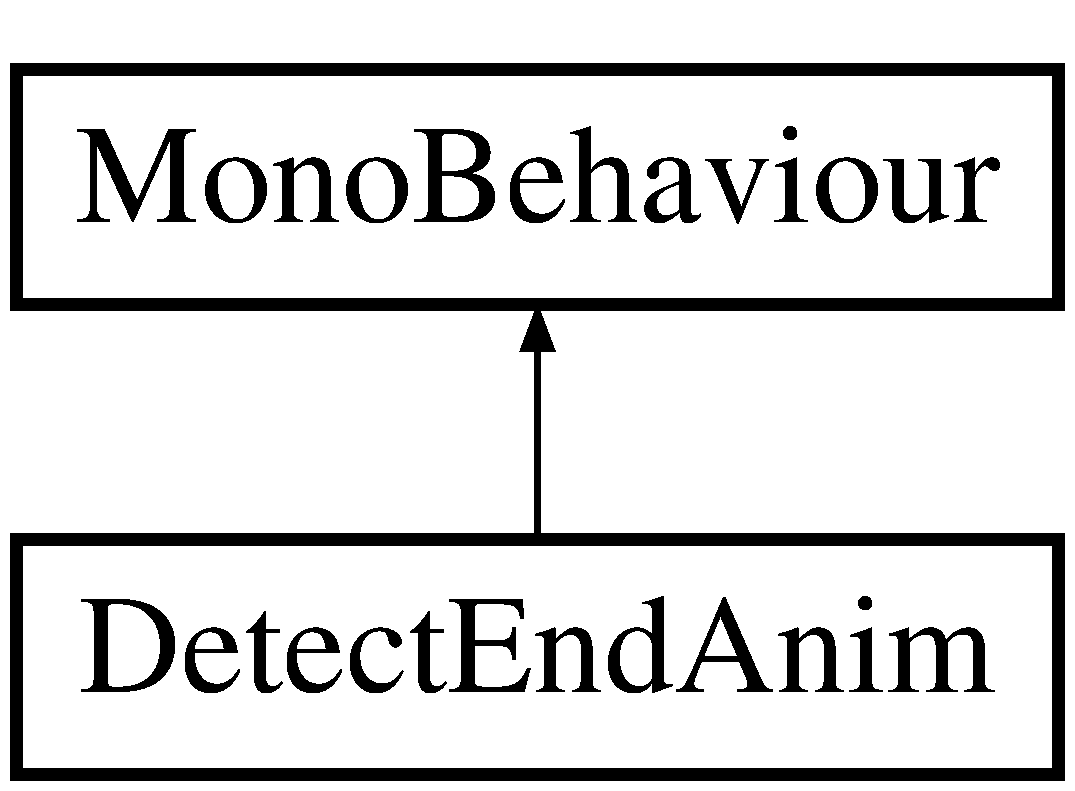
\includegraphics[height=2.000000cm]{class_detect_end_anim}
\end{center}
\end{figure}
\subsection*{Public Member Functions}
\begin{DoxyCompactItemize}
\item 
\mbox{\Hypertarget{class_detect_end_anim_a3214b4b28520b3d0f1316d3aad54b581}\label{class_detect_end_anim_a3214b4b28520b3d0f1316d3aad54b581}} 
void {\bfseries anim\+Ended} ()
\end{DoxyCompactItemize}
\subsection*{Public Attributes}
\begin{DoxyCompactItemize}
\item 
\mbox{\Hypertarget{class_detect_end_anim_a280dbf8134eb19d6f9dd30af4375c832}\label{class_detect_end_anim_a280dbf8134eb19d6f9dd30af4375c832}} 
Game\+Object {\bfseries start\+Anim\+Bttn} = null
\end{DoxyCompactItemize}


The documentation for this class was generated from the following file\+:\begin{DoxyCompactItemize}
\item 
Detect\+End\+Anim.\+cs\end{DoxyCompactItemize}

\hypertarget{class_gardei___cam_pan}{}\section{Gardei\+\_\+\+Cam\+Pan Class Reference}
\label{class_gardei___cam_pan}\index{Gardei\+\_\+\+Cam\+Pan@{Gardei\+\_\+\+Cam\+Pan}}
Inheritance diagram for Gardei\+\_\+\+Cam\+Pan\+:\begin{figure}[H]
\begin{center}
\leavevmode
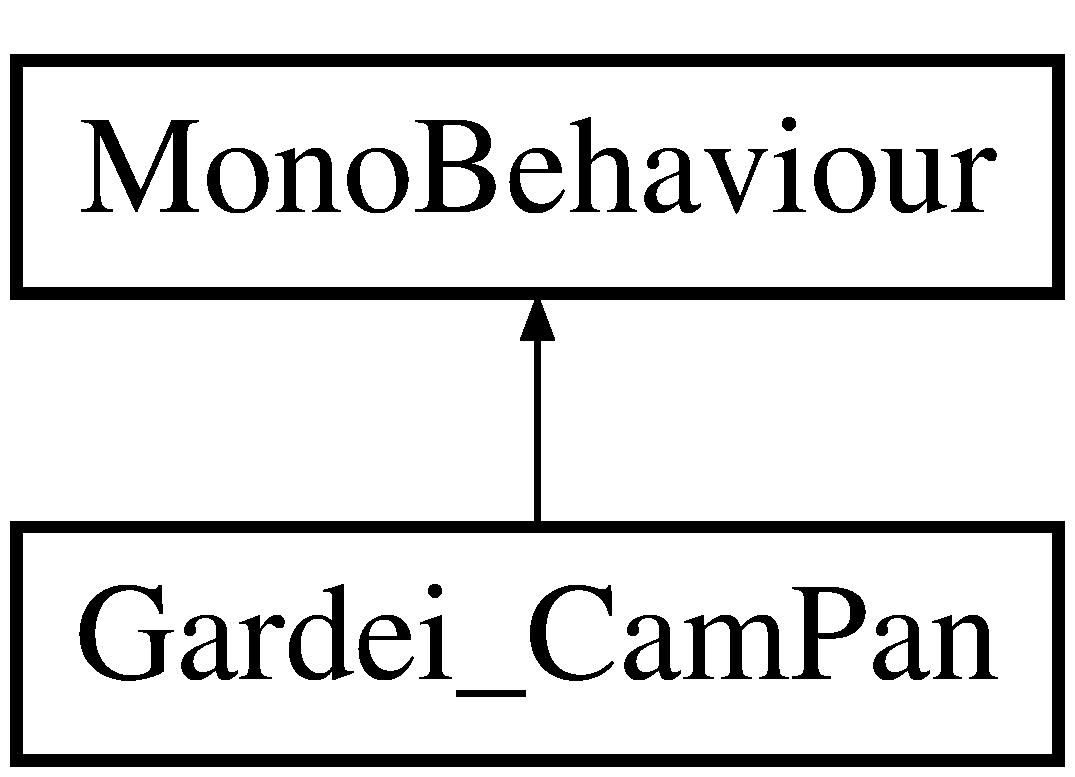
\includegraphics[height=2.000000cm]{class_gardei___cam_pan}
\end{center}
\end{figure}
\subsection*{Public Member Functions}
\begin{DoxyCompactItemize}
\item 
void \hyperlink{class_gardei___cam_pan_a3800f7be72b1b6b893e00e2c6248bcba}{set\+Target} (int station\+Num)
\begin{DoxyCompactList}\small\item\em Set\+Target\+: This function takes a target and will then immediately execute a camera transition as soon as it has been triggered. \end{DoxyCompactList}\item 
void \hyperlink{class_gardei___cam_pan_a6ae5373621faf797c67ad4eb961f40ca}{pan\+Cam} ()
\begin{DoxyCompactList}\small\item\em Resets the \char`\"{}lerp\char`\"{} code so the transition will start over from the current position. \end{DoxyCompactList}\end{DoxyCompactItemize}
\subsection*{Public Attributes}
\begin{DoxyCompactItemize}
\item 
Game\+Object \hyperlink{class_gardei___cam_pan_a22ff78b430a317e7871a396f35b097e6}{cam\+Pos1}
\begin{DoxyCompactList}\small\item\em cam\+Pos1\+: Target lerp position for station 1. cam\+Pos2\+: Target lerp position for station 2. cam\+Pos3\+: Target lerp position for station 3. cam\+Pos4\+: Target lerp position for station 4. cam\+Pos5\+: Target lerp position for station 5. cam\+Pos6\+: Target lerp position for station 6. cam\+Pos7\+: Target lerp position for station 7. cam\+Pos\+Sky\+: Target lerp position for Skyview. cam\+Pos\+H\+MI\+: Target lerp position for H\+MI. prior\+Pos\+: position of camera on last frame prior\+Rot\+: rotation of camera on last frame target\+Pos\+: position of target destination for camera target\+Rot\+: rotation of target rotation for camera move\+Cam\+: yes/no is the camera transitioning to a new position. lerp\+Time\+: maximum value of a lerp sequence. current\+Lerp\+Time\+: value between 0 and 1 will guide the camera through a transition to a new location. \end{DoxyCompactList}\item 
\mbox{\Hypertarget{class_gardei___cam_pan_aa4cfc9789ca0088602358fea82ad51fa}\label{class_gardei___cam_pan_aa4cfc9789ca0088602358fea82ad51fa}} 
Game\+Object {\bfseries cam\+Pos2}
\item 
\mbox{\Hypertarget{class_gardei___cam_pan_a5d21560f6c457bc96518f09db74f6a6d}\label{class_gardei___cam_pan_a5d21560f6c457bc96518f09db74f6a6d}} 
Game\+Object {\bfseries cam\+Pos3}
\item 
\mbox{\Hypertarget{class_gardei___cam_pan_ac6e127172963ce5e0300c145637e7838}\label{class_gardei___cam_pan_ac6e127172963ce5e0300c145637e7838}} 
Game\+Object {\bfseries cam\+Pos4}
\item 
\mbox{\Hypertarget{class_gardei___cam_pan_a5454f0988f8e6290c468a25741f82456}\label{class_gardei___cam_pan_a5454f0988f8e6290c468a25741f82456}} 
Game\+Object {\bfseries cam\+Pos5}
\item 
\mbox{\Hypertarget{class_gardei___cam_pan_a569365c3a56003d9e0208b3043d4623d}\label{class_gardei___cam_pan_a569365c3a56003d9e0208b3043d4623d}} 
Game\+Object {\bfseries cam\+Pos6}
\item 
\mbox{\Hypertarget{class_gardei___cam_pan_a4d524c86c24d5bb5a1582015c851cf88}\label{class_gardei___cam_pan_a4d524c86c24d5bb5a1582015c851cf88}} 
Game\+Object {\bfseries cam\+Pos7}
\item 
\mbox{\Hypertarget{class_gardei___cam_pan_a36c938a200942175f96689573de1335b}\label{class_gardei___cam_pan_a36c938a200942175f96689573de1335b}} 
Game\+Object {\bfseries cam\+Pos\+Sky}
\item 
\mbox{\Hypertarget{class_gardei___cam_pan_ad010b6b5ec0254cc2fd93c04a8062353}\label{class_gardei___cam_pan_ad010b6b5ec0254cc2fd93c04a8062353}} 
Game\+Object {\bfseries cam\+Pos\+H\+MI}
\end{DoxyCompactItemize}


\subsection{Member Function Documentation}
\mbox{\Hypertarget{class_gardei___cam_pan_a6ae5373621faf797c67ad4eb961f40ca}\label{class_gardei___cam_pan_a6ae5373621faf797c67ad4eb961f40ca}} 
\index{Gardei\+\_\+\+Cam\+Pan@{Gardei\+\_\+\+Cam\+Pan}!pan\+Cam@{pan\+Cam}}
\index{pan\+Cam@{pan\+Cam}!Gardei\+\_\+\+Cam\+Pan@{Gardei\+\_\+\+Cam\+Pan}}
\subsubsection{\texorpdfstring{pan\+Cam()}{panCam()}}
{\footnotesize\ttfamily void Gardei\+\_\+\+Cam\+Pan.\+pan\+Cam (\begin{DoxyParamCaption}{ }\end{DoxyParamCaption})}



Resets the \char`\"{}lerp\char`\"{} code so the transition will start over from the current position. 

\mbox{\Hypertarget{class_gardei___cam_pan_a3800f7be72b1b6b893e00e2c6248bcba}\label{class_gardei___cam_pan_a3800f7be72b1b6b893e00e2c6248bcba}} 
\index{Gardei\+\_\+\+Cam\+Pan@{Gardei\+\_\+\+Cam\+Pan}!set\+Target@{set\+Target}}
\index{set\+Target@{set\+Target}!Gardei\+\_\+\+Cam\+Pan@{Gardei\+\_\+\+Cam\+Pan}}
\subsubsection{\texorpdfstring{set\+Target()}{setTarget()}}
{\footnotesize\ttfamily void Gardei\+\_\+\+Cam\+Pan.\+set\+Target (\begin{DoxyParamCaption}\item[{int}]{station\+Num }\end{DoxyParamCaption})}



Set\+Target\+: This function takes a target and will then immediately execute a camera transition as soon as it has been triggered. 


\begin{DoxyParams}{Parameters}
{\em station\+Num} & integer that will tell the camera which preset position it needs to go to.\\
\hline
\end{DoxyParams}


\subsection{Member Data Documentation}
\mbox{\Hypertarget{class_gardei___cam_pan_a22ff78b430a317e7871a396f35b097e6}\label{class_gardei___cam_pan_a22ff78b430a317e7871a396f35b097e6}} 
\index{Gardei\+\_\+\+Cam\+Pan@{Gardei\+\_\+\+Cam\+Pan}!cam\+Pos1@{cam\+Pos1}}
\index{cam\+Pos1@{cam\+Pos1}!Gardei\+\_\+\+Cam\+Pan@{Gardei\+\_\+\+Cam\+Pan}}
\subsubsection{\texorpdfstring{cam\+Pos1}{camPos1}}
{\footnotesize\ttfamily Game\+Object Gardei\+\_\+\+Cam\+Pan.\+cam\+Pos1}



cam\+Pos1\+: Target lerp position for station 1. cam\+Pos2\+: Target lerp position for station 2. cam\+Pos3\+: Target lerp position for station 3. cam\+Pos4\+: Target lerp position for station 4. cam\+Pos5\+: Target lerp position for station 5. cam\+Pos6\+: Target lerp position for station 6. cam\+Pos7\+: Target lerp position for station 7. cam\+Pos\+Sky\+: Target lerp position for Skyview. cam\+Pos\+H\+MI\+: Target lerp position for H\+MI. prior\+Pos\+: position of camera on last frame prior\+Rot\+: rotation of camera on last frame target\+Pos\+: position of target destination for camera target\+Rot\+: rotation of target rotation for camera move\+Cam\+: yes/no is the camera transitioning to a new position. lerp\+Time\+: maximum value of a lerp sequence. current\+Lerp\+Time\+: value between 0 and 1 will guide the camera through a transition to a new location. 



The documentation for this class was generated from the following file\+:\begin{DoxyCompactItemize}
\item 
Gardei\+\_\+\+Cam\+Pan.\+cs\end{DoxyCompactItemize}

\hypertarget{classon_end}{}\section{on\+End Class Reference}
\label{classon_end}\index{on\+End@{on\+End}}
Inheritance diagram for on\+End\+:\begin{figure}[H]
\begin{center}
\leavevmode
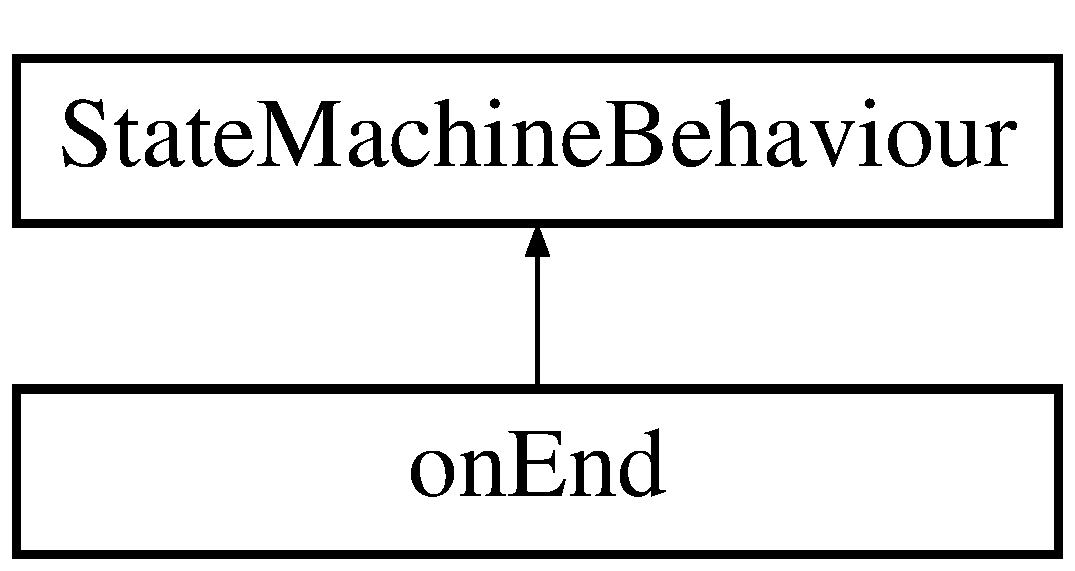
\includegraphics[height=2.000000cm]{classon_end}
\end{center}
\end{figure}
\subsection*{Public Member Functions}
\begin{DoxyCompactItemize}
\item 
\mbox{\Hypertarget{classon_end_a0e085abec95b7177c87310660196377d}\label{classon_end_a0e085abec95b7177c87310660196377d}} 
override void {\bfseries On\+State\+Update} (Animator anim, Animator\+State\+Info info, int index)
\item 
\mbox{\Hypertarget{classon_end_a4154e5dd9fe74d881feb2e0bbfc931ab}\label{classon_end_a4154e5dd9fe74d881feb2e0bbfc931ab}} 
override void {\bfseries On\+State\+Exit} (Animator anim, Animator\+State\+Info info, int index)
\end{DoxyCompactItemize}


The documentation for this class was generated from the following file\+:\begin{DoxyCompactItemize}
\item 
on\+End.\+cs\end{DoxyCompactItemize}

\hypertarget{class_world_controller}{}\section{World\+Controller Class Reference}
\label{class_world_controller}\index{World\+Controller@{World\+Controller}}
Inheritance diagram for World\+Controller\+:\begin{figure}[H]
\begin{center}
\leavevmode
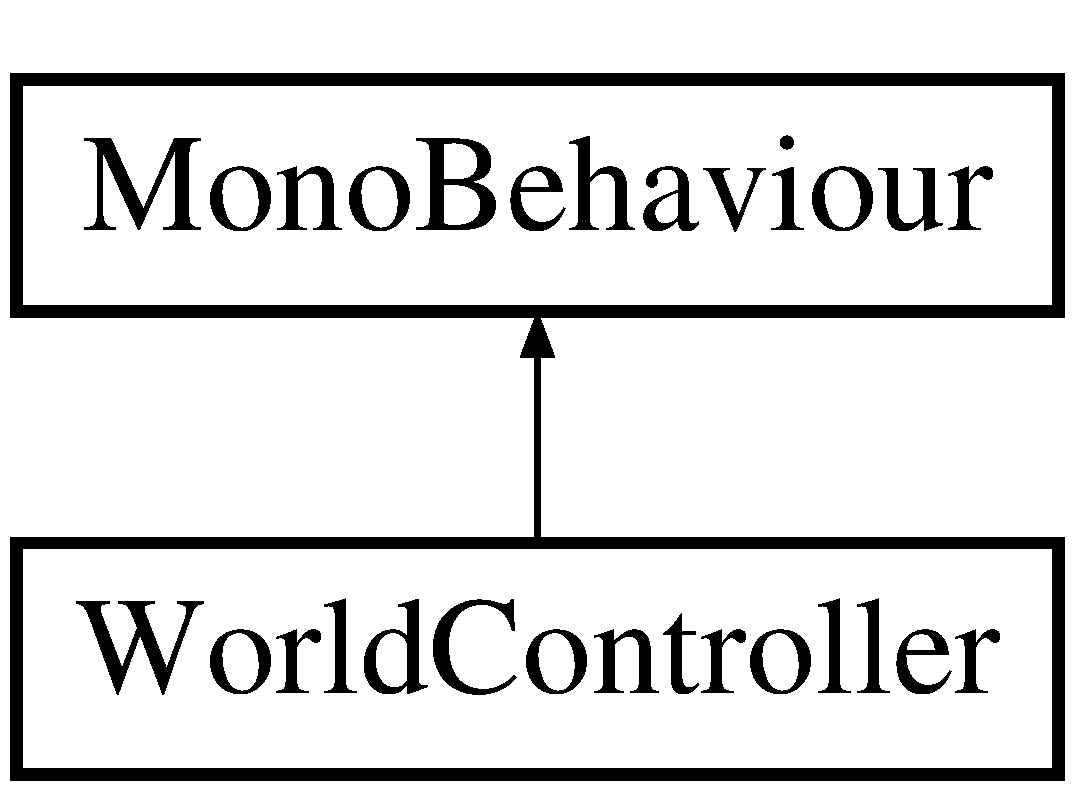
\includegraphics[height=2.000000cm]{class_world_controller}
\end{center}
\end{figure}
\subsection*{Public Member Functions}
\begin{DoxyCompactItemize}
\item 
\mbox{\Hypertarget{class_world_controller_a16dd47d6cb47d7e9f4fbd1b70e597afd}\label{class_world_controller_a16dd47d6cb47d7e9f4fbd1b70e597afd}} 
void {\bfseries anim\+Start} ()
\item 
\mbox{\Hypertarget{class_world_controller_ab03bc22973aba3a5fda4000f5ba7159e}\label{class_world_controller_ab03bc22973aba3a5fda4000f5ba7159e}} 
void {\bfseries anim\+Ended} ()
\end{DoxyCompactItemize}
\subsection*{Public Attributes}
\begin{DoxyCompactItemize}
\item 
\mbox{\Hypertarget{class_world_controller_a94e5f3a146e639dc2d6156470313f7b9}\label{class_world_controller_a94e5f3a146e639dc2d6156470313f7b9}} 
Animator {\bfseries machine\+\_\+1}
\item 
\mbox{\Hypertarget{class_world_controller_a093c7db83872c7d8b09a1c67937ae121}\label{class_world_controller_a093c7db83872c7d8b09a1c67937ae121}} 
Game\+Object {\bfseries start\+Anim\+Bttn} = null
\end{DoxyCompactItemize}


The documentation for this class was generated from the following file\+:\begin{DoxyCompactItemize}
\item 
World\+Controller.\+cs\end{DoxyCompactItemize}

%--- End generated contents ---

% Index
\backmatter
\newpage
\phantomsection
\clearemptydoublepage
\addcontentsline{toc}{chapter}{Index}
\printindex

\end{document}
